\section{Scale Recovery}

\subsection{How to recover global position and scale?}
With a single camera, \textbf{monocular visual odometry} (VO) recovers the motion and the structure of the scene only up to a \textbf{similarity transform}. The whole reconstruction can be rotated, translated and \emph{scaled} without changing the images. A small scene seen from close and a big scene seen from far away produce exactly the same pictures. As a consequence:
\begin{compactitemize}
    \item the \textbf{absolute scale} (how many metres a unit of the reconstruction is) is not observable from images alone;
    \item the \textbf{absolute global position} (where we are in the world) is not observable from images alone either.
\end{compactitemize}

In practice the problem is fixed by adding \textbf{other sensors or priors}:
\begin{compactitemize}
    \item a stereo or depth camera, which measures the depth directly;
    \item an \textbf{IMU} (visual-inertial odometry), which measures accelerations in m/s$^2$;
    \item objects of known size in the scene;
    \item GPS, which also gives the global position.
\end{compactitemize}
In this chapter we analyze how to fuse the \textbf{Inertial Measurement Unit (IMU)} with the other sensors to enable scale recovery.

\subsection{What is an IMU?}
An inertial measurement unit typically combines two sensors.

The \textbf{three-axis gyroscope} measures the \textbf{angular velocity} of the sensor frame relative to an inertial frame, in rad/s:
\[
\omega_m = \omega + b_g + n_g
\]

The \textbf{three-axis accelerometer} measures the \textbf{specific force}, i.e.\ the non-gravitational acceleration expressed in the sensor frame, in m/s$^2$:
\[
a_m = f + b_a + n_a
\]

In both cases the measurement is the true value plus a bias ($b$) and a noise ($n$), which are described in Section~\ref{sec:imu-model}. The IMU reports its measurements in its own \textbf{body/sensor coordinate frame}, not directly in the world frame. To use them for navigation, we must therefore know the orientation of the sensor.

The accelerometer measures \emph{acceleration}, i.e.\ a quantity with a physical unit (m/s$^2$). This is why the IMU makes the scale observable: by integrating it twice we get displacements in metres, which fix the unknown scale of monocular VO.

\subsection{Gravity}
Let $W$ be the world frame and $B$ the IMU frame, and let $R_{WB}$ rotate vectors from $B$ to $W$. Newton's law gives the acceleration in the world frame as the sum of gravity and the specific force:
\[
a_W = g_W + R_{WB}\, f_B
\]
hence the accelerometer measures:
\[
\boxed{f_B = R_{WB}^T \left(a_W - g_W\right)}
\]

At rest $a_W = 0$, so the accelerometer measures
\[
f_B = -R_{WB}^T\, g_W
\]
which has magnitude approximately $g$. An accelerometer lying still on a table does \emph{not} read zero: it reads about $9.81\,\mathrm{m/s^2}$ pointing \emph{upwards}, which is the reaction force of the table that prevents it from falling. For this reason gravity must always be removed, and this requires knowing the orientation $R_{WB}$.

\subsection{Frames, states and sign conventions}
We use a common visual-inertial / factor-graph convention:
\begin{compactitemize}
    \item $W$ is the world frame and $B$ the IMU/body frame;
    \item $R_k \equiv R_{WB_k} \in SO(3)$ maps body-frame vectors to the world frame;
    \item $p_k, v_k \in \mathbb{R}^3$ are the world-frame position and velocity;
    \item $g_W$ is constant in the world frame, e.g.\ $(0, 0, -g)^T$ with the $z$ axis up;
    \item $\omega_m, a_m$ are sampled in the body frame.
\end{compactitemize}
The \textbf{continuous-time ideal kinematics} are:
\[
\dot R_{WB} = R_{WB}\, [\omega]_\times, \qquad
\dot v_W = g_W + R_{WB}\, f_B, \qquad
\dot p_W = v_W
\]
The orientation changes with the angular velocity, the velocity changes with the specific force (rotated into the world) plus gravity, and the position changes with the velocity.

\subsection{A practical IMU measurement model}\label{sec:imu-model}
The measured signals are modeled as:
\[
\begin{aligned}
\omega_m(t) &= \omega(t) + b_g(t) + n_g(t)\\
a_m(t) &= f(t) + b_a(t) + n_a(t)
\end{aligned}
\]
where:
\begin{compactitemize}
    \item $\omega, f$ are the true angular velocity and specific force;
    \item $b_g, b_a$ are the gyroscope and accelerometer \textbf{biases};
    \item $n_g, n_a$ are the high-frequency \textbf{measurement noise}.
\end{compactitemize}

The bias is \textbf{not} the same as white measurement noise:
\begin{compactitemize}
    \item \textbf{white noise} changes rapidly and is often modeled as independent samples;
    \item the \textbf{bias} changes slowly and is correlated over time.
\end{compactitemize}

A more complete sensor model can also include scale-factor errors, axis misalignment, non-orthogonality of the axes, temperature dependence, saturation, quantization and timing errors.

\subsubsection{Bias: a persistent measurement offset}
Suppose the true signal is zero and the sensor has a constant bias:
\[
y_m(t) = b + n(t)
\]
Even if the noise $n(t)$ averages to zero, the \textbf{mean measurement tends to $b$}, not to zero. Averaging more samples removes the noise but not the bias. This is the same idea as the bias in the RMSE decomposition of Section~\ref{sec:least-squares}.

\begin{figure}[H]
    \centering
    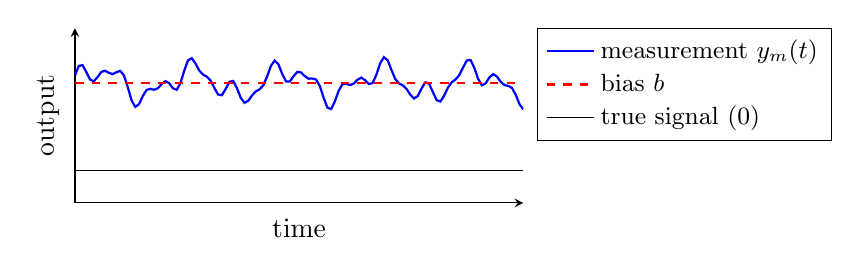
\begin{tikzpicture}
    \begin{axis}[
        width=0.6\textwidth, height=3.8cm,
        axis lines=left, xlabel={time}, ylabel={output},
        xtick=\empty, ytick=\empty, xmin=0, xmax=10, ymin=-0.3, ymax=1.3,
        samples=120, legend pos=outer north east, legend cell align=left, legend style={font=\small}]
        \addplot[blue, thick, domain=0:10] {0.8 + 0.12*sin(deg(3*x)) + 0.08*sin(deg(7.3*x+1)) + 0.05*sin(deg(13*x))};
        \addlegendentry{measurement $y_m(t)$}
        \addplot[red, dashed, thick, domain=0:10] {0.8};
        \addlegendentry{bias $b$}
        \addplot[black, thin, domain=0:10] {0};
        \addlegendentry{true signal (0)}
    \end{axis}
    \end{tikzpicture}
    \caption{A biased sensor: the measurement oscillates around $b$, not around the true value $0$}
\end{figure}

The bias is dangerous because the IMU measurements are \textbf{integrated}:
\begin{compactitemize}
    \item the \textbf{gyroscope bias} integrates into an \textbf{attitude error};
    \item the \textbf{accelerometer bias} integrates into \textbf{velocity and position errors}.
\end{compactitemize}
Bias calibration is therefore essential for inertial navigation.

\subsubsection{Bias drift: a stochastic process}
The bias is not perfectly constant: it slowly drifts. A widely used model is the \textbf{first-order random walk}:
\[
\dot b(t) = n_b(t)
\]
where $n_b$ is continuous-time white noise with spectral density $Q_b$:
\[
\mathbb{E}[n_b(t)] = 0, \qquad \mathbb{E}\!\left[n_b(t)\, n_b(\tau)^T\right] = Q_b\, \delta(t-\tau)
\]
Over a sample interval $\Delta t$ this becomes:
\[
b_{k+1} = b_k + w_{b,k}, \qquad w_{b,k} \sim \mathcal{N}(0,\, Q_b\, \Delta t)
\]
So the bias is approximately constant over short intervals, but its uncertainty \textbf{grows with the elapsed time}:
\[
\operatorname{Cov}\!\left(b(t) - b(0)\right) = Q_b\, t
\]

\begin{infobox}[Interpretation]
Bias drift is not necessarily a deterministic trend, i.e.\ the bias does not simply grow in one direction. It is modeled as a slow stochastic variation whose increments are independent. We cannot predict where the bias will go, but we know how much it can move in a given time.
\end{infobox}

\begin{infobox}[Brownian motion]
The random walk $\dot b = n_b$ is the mathematical model of \textbf{Brownian motion}, the erratic motion of a small particle in a fluid, which is continuously hit by the molecules around it. The integral of white noise is called a \textbf{Wiener process}. Its main properties are the same as those of the bias:
\begin{compactitemize}
    \item the increments over disjoint time intervals are \textbf{independent} and Gaussian, with zero mean;
    \item the expected value stays at the starting point, $\mathbb{E}[b(t)] = b(0)$, so on average the bias does not move;
    \item the variance grows \textbf{linearly} with time, $\operatorname{Var} = Q_b\, t$, so the typical distance from the start grows as $\sqrt{t}$.
\end{compactitemize}
Like a Brownian particle, the bias wanders without a preferred direction. We cannot predict where it will be, only how far it can typically go. For this reason the bias is kept in the state and re-estimated continuously.
\end{infobox}

\subsubsection{How biases create navigation drift}
Consider a one-dimensional motion, initially at rest, with a constant accelerometer bias $b_a$ and no other errors:
\[
\hat a(t) = a(t) + b_a
\]
Integrating once, the velocity error grows \textbf{linearly}:
\[
\delta v(t) = \int_0^t b_a\, d\tau = b_a\, t
\]
Integrating again, the position error grows \textbf{quadratically}:
\[
\boxed{\delta p(t) = \int_0^t \delta v(\tau)\, d\tau = \frac{1}{2}\, b_a\, t^2}
\]
For a constant gyroscope bias $b_g$, the small-angle attitude error grows approximately linearly:
\[
\delta\theta(t) \simeq b_g\, t
\]
A wrong attitude is even worse than it looks: with a wrong $R_{WB}$, gravity is not removed correctly, and part of $g$ leaks into the horizontal acceleration, which is then integrated twice as well.

\begin{examplebox}[Numerical intuition: a tiny bias gives a large error]
Consider a constant accelerometer bias of only $1\,\mathrm{m}g$:
\[
b_a = 0.001\, g \simeq 9.81 \times 10^{-3}\ \mathrm{m/s^2}
\]
\begin{center}
\begin{tabular}{c|c|c}
$t$ & $\delta v = b_a t$ & $\delta p = \frac{1}{2} b_a t^2$ \\ \hline
10 s & 0.098 m/s & 0.49 m \\
30 s & 0.294 m/s & 4.41 m \\
60 s & 0.589 m/s & 17.66 m
\end{tabular}
\end{center}
After only one minute the position is wrong by almost 18 metres. These values are for an isolated constant bias, without any aiding sensor or feedback correction.
\end{examplebox}

\textbf{Why sensor fusion helps.} GNSS, vision, LiDAR, radar, wheel odometry and motion constraints periodically \textbf{correct the inertial drift}. With suitable motion, they also make the biases \textbf{observable}, so that the biases can be estimated online together with the trajectory.

\subsection{Continuous-time inertial navigation}
Substituting the measurement model into the motion equations (i.e.\ replacing the true $\omega$ and $f$ with the measured values minus bias and noise) we get:
\[
\begin{aligned}
\dot p_W &= v_W\\
\dot v_W &= g_W + R_{WB}\left(a_m - b_a - n_a\right)\\
\dot R_{WB} &= R_{WB}\left[\omega_m - b_g - n_g\right]_\times\\
\dot b_g &= n_{wg}\\
\dot b_a &= n_{wa}
\end{aligned}
\]
The state is:
\[
x = \left(R,\ v,\ p,\ b_g,\ b_a\right)
\]
The first three equations propagate the \textbf{navigation state}, while the last two describe the slow \textbf{bias evolution} (random walk).

\subsection{Discrete-time propagation}
The IMU gives samples, not continuous signals. We assume that the measurements and the biases are approximately constant over $[t_k, t_{k+1}]$, with $\Delta t = t_{k+1} - t_k$, and define the bias-corrected measurements:
\[
\hat\omega_k = \omega_{m,k} - b_{g,k}, \qquad \hat f_k = a_{m,k} - b_{a,k}
\]
Using a zero-order hold and a first-order integration:
\[
\begin{aligned}
R_{k+1} &\simeq R_k\, \operatorname{Exp}\!\left(\hat\omega_k\, \Delta t\right)\\
v_{k+1} &\simeq v_k + \left(g_W + R_k \hat f_k\right) \Delta t\\
p_{k+1} &\simeq p_k + v_k\, \Delta t + \frac{1}{2}\left(g_W + R_k \hat f_k\right) \Delta t^2
\end{aligned}
\]
The rotation is updated with the exponential map ($\operatorname{Exp}$) seen in Section~\ref{sec:least-squares}, so that it stays a valid rotation. This is a simple discrete integrator. \textbf{Midpoint integration} improves the accuracy when the angular velocity or the specific force changes appreciably within a sample.

\subsection{IMU preintegration}
\subsubsection{Why integrate between keyframes?}
A camera, LiDAR or radar \textbf{keyframe} may be available at a much lower rate than the IMU. Between two keyframes $i$ and $j$ there may be hundreds of IMU samples.

\begin{figure}[H]
    \centering
    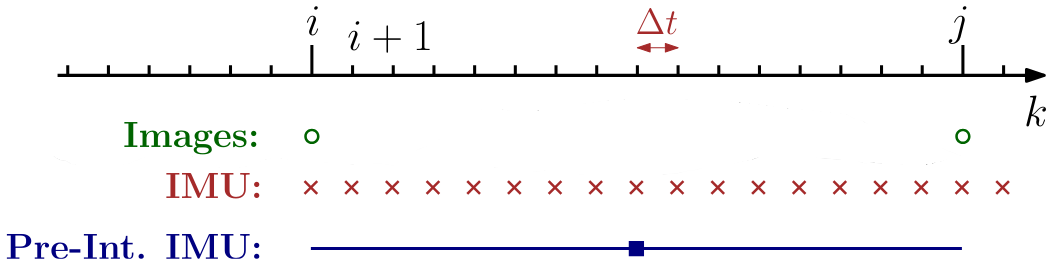
\includegraphics[width=0.7\textwidth]{images/C11_1.png}
    \caption{Images arrive only at the keyframes $i$ and $j$, while the IMU gives many samples in between. Preintegration summarizes them in a single relative measurement}
\end{figure}

In the factor graph, the states are only the keyframes. During the optimization the estimates of the keyframe states change at every iteration. If the IMU integration starts from the estimated pose and velocity at keyframe $i$, all the samples between $i$ and $j$ would have to be \textbf{re-integrated} after every update, which is very expensive. \textbf{Preintegration} solves this problem: it builds a \textbf{relative-motion summary} that does not depend on the global pose and velocity at keyframe $i$. It is computed once, and then reused at every iteration.

\subsubsection{Preintegrated measurements}
We assume that measurements and biases are approximately constant over $[t_i, t_j]$, with $N$ IMU samples in this range, and define the measurements corrected with the nominal biases $\bar b_g, \bar b_a$:
\[
\omega_k = \omega_{m,k} - \bar b_g, \qquad a_k = a_{m,k} - \bar b_a, \qquad \Delta t = t_{k+1} - t_k
\]
Chaining the discrete propagation from $i$ to $j$, we get three equations. In each one, the part that depends only on the IMU samples can be separated from the states at time $i$. These parts are the \textbf{preintegrated measurements} $\gamma_{ij}, \beta_{ij}, \alpha_{ij}$.

\textbf{Rotation:}
\[
R_j = R_i \prod_{k=0}^{N} \operatorname{Exp}\!\left(\omega_k \Delta t\right) = R_i\, \gamma_{ij}
\]

\textbf{Velocity:}
\[
v_j = v_i + g\,(t_j - t_i) + R_i \sum_{k=0}^{N} \Delta R_{ik}\, a_k\, \Delta t = v_i + g\,(t_j - t_i) + R_i\, \beta_{ij}
\]

\textbf{Position:}
\[
\begin{aligned}
p_j &= p_i + v_i\,(t_j - t_i) + \frac{1}{2} g\,(t_j - t_i)^2 + R_i \sum_{k=0}^{N} \left(\beta_{ik}\, \Delta t + \frac{1}{2} \Delta R_{ik}\, a_k\, \Delta t^2\right)\\
&= p_i + v_i\,(t_j - t_i) + \frac{1}{2} g\,(t_j - t_i)^2 + R_i\, \alpha_{ij}
\end{aligned}
\]
Here $\Delta R_{ik} = R_i^T R_k$ is the rotation accumulated from $i$ to sample $k$. It is computed from the gyroscope samples only, so the sums do not depend on the global orientation $R_i$. In the position, $\beta_{ik}$ is the velocity change preintegrated up to sample $k$: at each step the position grows both with the velocity already accumulated and with the new acceleration.

So $\gamma_{ij}$ is the relative rotation, $\beta_{ij}$ the velocity change and $\alpha_{ij}$ the position change, all expressed in the frame of keyframe $i$ and without gravity.

\subsubsection{Preintegration residuals}
Solving the three equations for the preintegrated quantities, we get what the \textbf{states} predict for them:
\[
\begin{aligned}
\alpha_{ij} &= R_i^T \left(p_j - p_i - v_i\,(t_j - t_i) - \frac{1}{2} g\,(t_j - t_i)^2\right)\\
\beta_{ij} &= R_i^T \left(v_j - v_i - g\,(t_j - t_i)\right)\\
\gamma_{ij} &= R_i^T R_j
\end{aligned}
\]
The bias random walk adds two more constraints. Over a short interval the biases are almost constant:
\[
0 = b_{a,j} - b_{a,i}, \qquad 0 = b_{g,j} - b_{g,i}
\]
The \textbf{residuals} are the differences between the values predicted by the states and the values measured by preintegration. For the rotation the difference is computed on the manifold, with the logarithm map:
\[
\begin{aligned}
r_R &= \operatorname{Log}\!\left(\tilde\gamma_{ij}^T\, R_i^T R_j\right)\\
r_v &= R_i^T \left(v_j - v_i - g\,(t_j - t_i)\right) - \tilde\beta_{ij}\\
r_p &= R_i^T \left(p_j - p_i - v_i\,(t_j - t_i) - \tfrac{1}{2} g\,(t_j - t_i)^2\right) - \tilde\alpha_{ij}\\
r_{b_g} &= b_{g,j} - b_{g,i}\\
r_{b_a} &= b_{a,j} - b_{a,i}
\end{aligned}
\]
where $\tilde\gamma_{ij}, \tilde\beta_{ij}, \tilde\alpha_{ij}$ are the values computed from the IMU samples.

\begin{figure}[H]
    \centering
    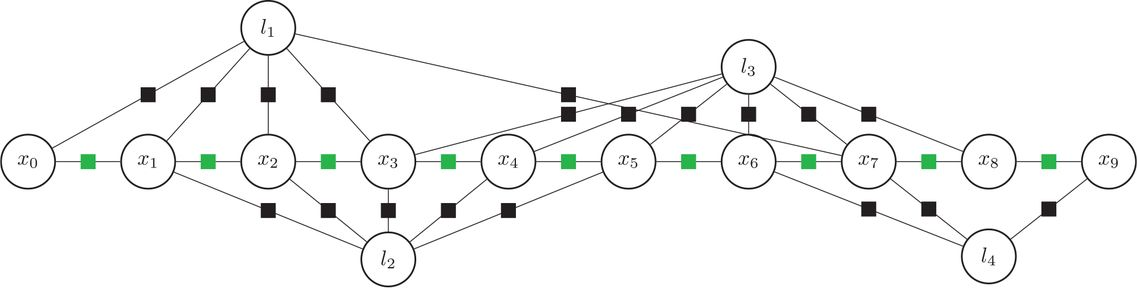
\includegraphics[width=0.85\textwidth]{images/C10_7.png}
    \caption{VIO factor graph: the IMU preintegration factors (green) connect consecutive keyframes $x_i$, and the reprojection factors (black) connect keyframes and landmarks $l_j$}
    \label{fig:vio-graph-imu}
\end{figure}

\subsubsection{The complete 15-dimensional IMU residual}
Stacking the five residuals, each of dimension 3, we get the complete IMU residual:
\[
r_{ij} = \begin{bmatrix} r_R \\ r_v \\ r_p \\ r_{b_g} \\ r_{b_a} \end{bmatrix} \in \mathbb{R}^{15}
\]

\begin{infobox}[Residuals with different units need weights]
At this point the cost function contains residuals measured in \textbf{different units}. Inside the IMU residual alone, $r_R$ is in radians, $r_v$ in m/s and $r_p$ in metres. In VIO we also add the reprojection residuals of the camera, which are in \textbf{pixels}. Summing them directly makes no sense: an error of 1 pixel and an error of 1 metre are not equivalent, so a minimization done in metres cannot be compared with one done in pixels. Moreover, the result would change just by changing the units, e.g.\ from metres to millimetres.

For this reason we must \textbf{weight} each residual, as in weighted least squares (Section~\ref{sec:least-squares}). The natural weight is the inverse of the \textbf{covariance} $\Sigma$ of the measurement, which gives the \textbf{Mahalanobis norm}:
\[
\left\| r \right\|_{\Sigma}^2 = r^T\, \Sigma^{-1}\, r
\]
The total cost then becomes:
\[
\min \ \sum_{i,j} \left\| r^{cam}_{ij} \right\|^2_{\Sigma_{cam}} + \sum_{i} \left\| r^{IMU}_{i,i+1} \right\|^2_{\Sigma_{IMU}} + \dots
\]
Dividing each residual by its standard deviation makes it \textbf{dimensionless}. It now counts ``how many sigmas'' the error is, so residuals of different sensors become comparable. A precise sensor (small $\Sigma$) gets a large weight, and a noisy one gets a small weight, exactly like $w_i = 1/\sigma_i^2$. For the IMU factor, the covariance $\Sigma_{IMU}$ ($15\times15$) is propagated together with the preintegrated quantities, starting from the noise densities of the gyroscope and the accelerometer and from the bias random walk.
\end{infobox}

\subsubsection{Why preintegration needs bias correction}
The preintegrated quantities were computed using the \textbf{nominal biases} $(\bar b_g, \bar b_a)$. During the nonlinear optimization the estimated biases change:
\[
\delta b_g = b_g - \bar b_g, \qquad \delta b_a = b_a - \bar b_a
\]
Re-integrating every raw IMU sample after every optimizer update would be costly. Instead, the preintegrated quantities are approximated as \textbf{first-order functions} of the bias perturbations:
\[
\begin{aligned}
\gamma(b_g) &\simeq \gamma\, \operatorname{Exp}\!\left(J_{R,g}\, \delta b_g\right)\\
\beta(b_g, b_a) &\simeq \beta + J_{v,g}\, \delta b_g + J_{v,a}\, \delta b_a\\
\alpha(b_g, b_a) &\simeq \alpha + J_{p,g}\, \delta b_g + J_{p,a}\, \delta b_a
\end{aligned}
\]
The Jacobians are evaluated \textbf{during preintegration}, at the nominal biases, so they cost nothing extra. Note that the rotation depends only on the gyroscope bias, while velocity and position depend on both biases.

\subsection{What the IMU factor connects}
In the factor graph, the IMU factor is a factor between two consecutive keyframes:
\begin{compactitemize}
    \item it constrains the two keyframe states $(R, v, p)$ over the interval $[t_i, t_j]$;
    \item the biases at the first endpoint ($b_{g,i}, b_{a,i}$) determine the bias-corrected preintegration;
    \item the bias random-walk terms connect the biases of the two endpoints;
    \item the other sensors (camera, LiDAR, GPS, \dots) provide complementary constraints and help to bound the drift.
\end{compactitemize}
This is exactly the green odometry factor of the VIO factor graph of Section~\ref{sec:bundle-adjustment} (Figure~\ref{fig:vio-graph-imu}). The black reprojection factors connect the poses to the landmarks, and the IMU factors connect consecutive poses. The IMU factors make the scale observable, while the camera factors limit the drift of the IMU.



\subsection{Examples and what's next}
\begin{figure}[H]
    \centering
    \begin{subfigure}[b]{0.4\textwidth}
        \centering
        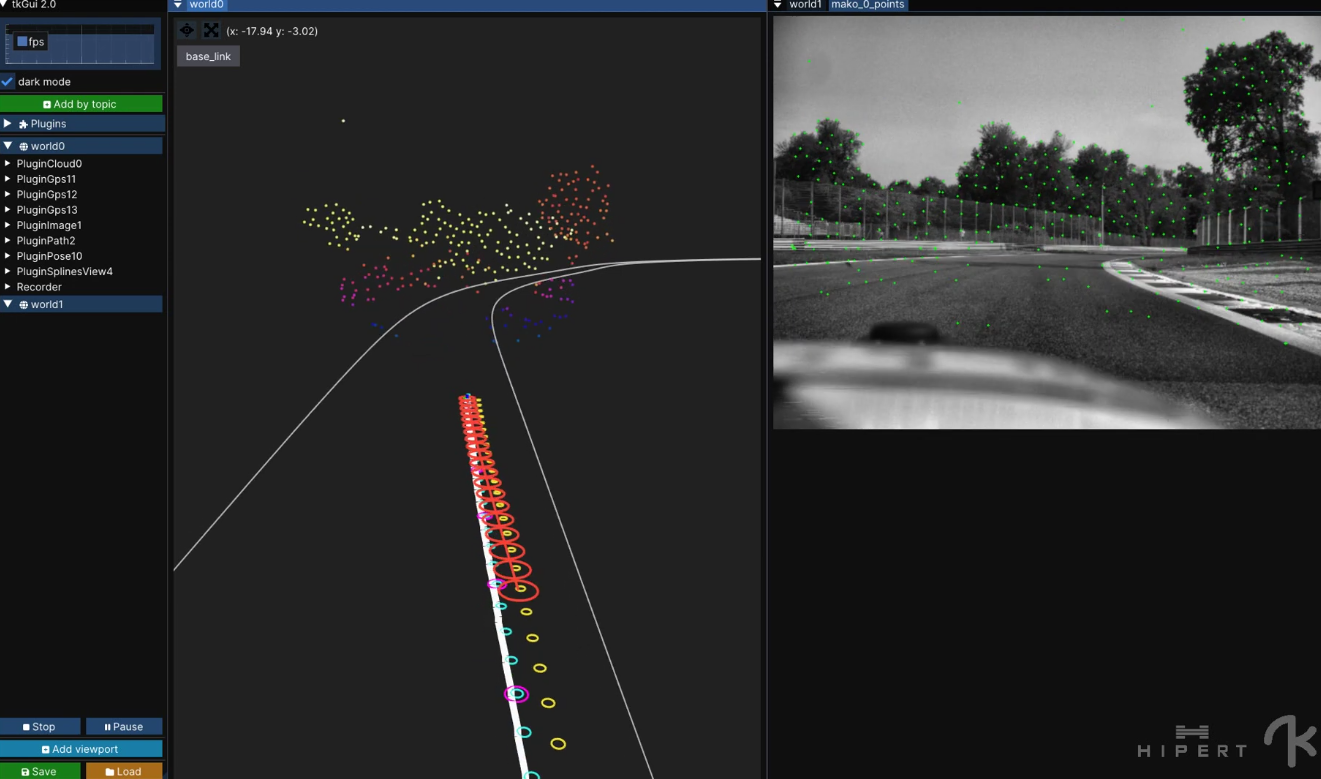
\includegraphics[width=\textwidth]{images/C11_2.png}
        \caption{VIO for autonomous racing}
    \end{subfigure}
    \hfill
    \begin{subfigure}[b]{0.4\textwidth}
        \centering
        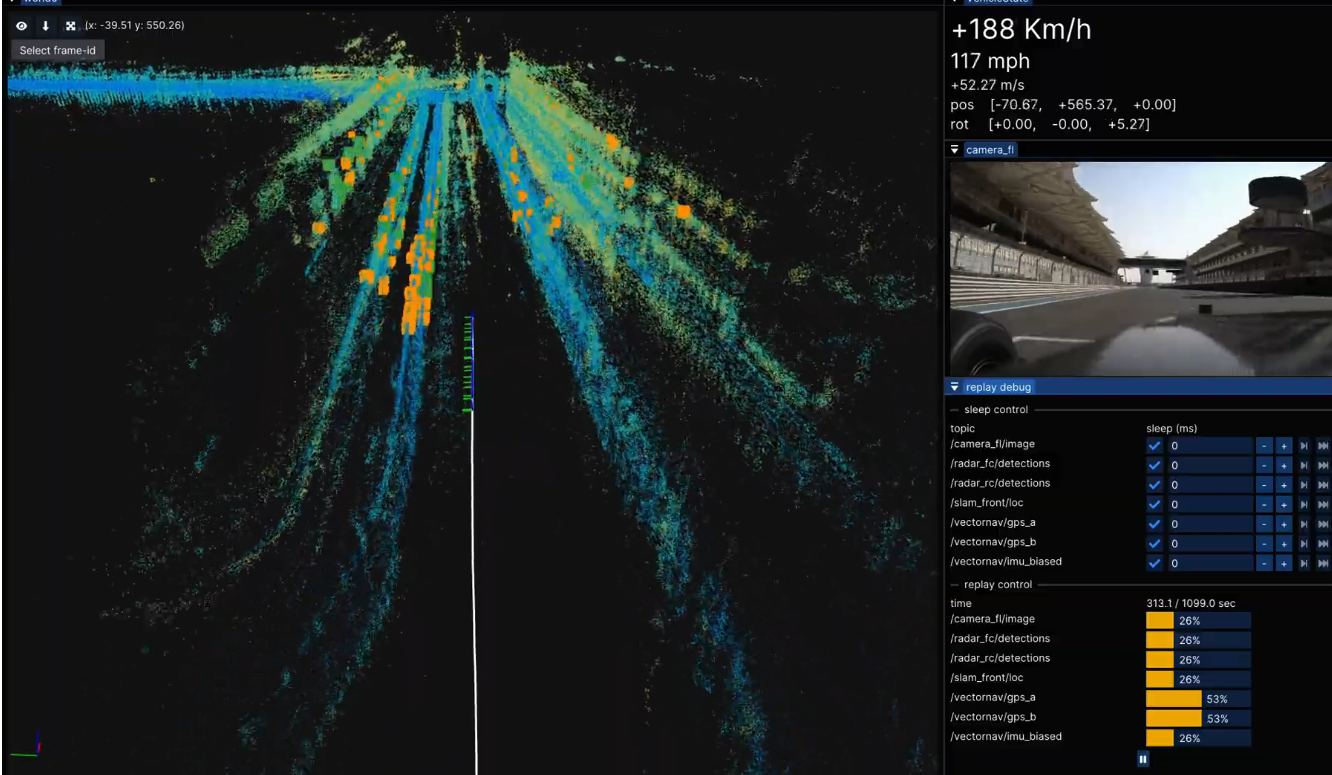
\includegraphics[width=\textwidth]{images/C11_3.png}
        \caption{Radar localization on a map}
    \end{subfigure}
    \caption{Examples shown in the course (videos)}
\end{figure}

The same estimation tools are used for several related problems:
\begin{compactitemize}
    \item \textbf{Odometry}: estimation of the vehicle's \textbf{relative motion} over time, typically by integrating measurements from onboard sensors such as cameras, LiDAR, radar or IMU. It drifts over time.
    \item \textbf{SLAM} (Simultaneous Localization and Mapping): joint estimation of the vehicle's trajectory and of the structure of an initially unknown environment, while building a map of it. It uses \textbf{loop closure} on the built map to correct the drift.
    \item \textbf{Mapping}: joint \textbf{offline} estimation of the vehicle trajectory and of the map, by optimizing a batch of measurements collected over a sequence. It typically uses all the measurements at the same time to obtain a globally consistent solution.
    \item \textbf{Localization on a map}: estimation of the vehicle's pose with respect to a \textbf{known, pre-existing map}, without necessarily modifying or reconstructing the map.
\end{compactitemize}

\subsubsection{What about other sensors?}
The same approach (a factor graph with a dedicated factor for each sensor) works with other sensors as well: LiDAR,radar,GNSS, thermal camera, event camera, etc.

